\documentclass[12pt, letter]{exam}
\usepackage[utf8]{inputenc}
\usepackage[T1]{fontenc}
\usepackage[spanish]{babel}
\usepackage[autostyle,spanish=mexican]{csquotes}
\usepackage{amsmath}
\usepackage{amsthm}
\usepackage{physics}
\usepackage{tikz}
\usepackage{float}
\usepackage{siunitx}
\usepackage{multicol}
\usepackage{paralist}
\usepackage{enumitem}
\usepackage[left=2.00cm, right=2.00cm, top=2.00cm, 
     bottom=2.00cm]{geometry}
\usepackage{pdfpages}
\usepackage{circuitikz}

% \renewcommand{\questionlabel}{\thequestion}
\decimalpoint

\setlength{\belowdisplayskip}{-0.5pt}

\usepackage{tasks}
\settasks{
    label=\Alph*), 
    label-align=left,
    item-indent={20pt}, 
    column-sep={4pt},
    label-width={16pt},
}

\sisetup{per-mode=symbol}
\footer{}{\thepage}{}

\begin{document}
\includepdf[pages={1}]{Caratula_Examen_Parcial_03_PU_Fisica_4_01.pdf}

\newpage

\begin{questions}
    
    \section{(6 puntos) Hidrodinámica.}

    \question \textbf{(1 punto)} En la hidrodinámica un fluido se considera ideal cuando:
    \begin{parts}
        \part La densidad es constante.
        \part Las fuerzas son no conservativas.
        \part Las partículas solo tienes movimiento de traslación.
        \part La temperatura del fluido varía con la velocidad.
    \end{parts}
    \question \textbf{(1 punto)} \label{Problema_01} \textbf{Ejercicio de ejecución: } En el cuerpo humano el flujo sanguíneo es de $5$ litros de sangre por minuto. ¿Cuál es el área de la sección transversal de la aorta, si la sangre en ese vaso tiene una velocidad de \SI{28}{\centi\meter\per\second}?
    \begin{tasks}(4)
        \task \SI{3.10}{\square\centi\meter}
        \task \SI{2.77}{\square\centi\meter}
        \task \SI{1.77}{\square\centi\meter}
        \task \SI{2.97}{\square\centi\meter}
    \end{tasks}
    \question \textbf{(1 punto)} Bernoulli al estudiar la relación entre la presión y la velocidad de un líquido que circula por una tubería, encontró que la presión es \rule{2cm}{0.1mm} si su velocidad es \rule{2cm}{0.1mm}:
    \begin{tasks}(4)
        \task alta - cero.
        \task baja - máxima.
        \task baja - alta.
        \task alta - alta.
    \end{tasks}
    \question \textbf{(1 punto)} La ecuación de Bernoulli que se muestra a continuación contiene tres términos de cada lado de la igualdad:
    \begin{align*}
    \underbrace{P_{1}}_{\text{\large{a}}} + \underbrace{\rho \, g \, h_{1}}_{\text{\large{b}}} + \underbrace{\dfrac{1}{2} \rho \, v_{1}^{2}}_{\text{\large{c}}} = P_{2} + \rho \, g \, h_{2} + \dfrac{1}{2} \rho \, v_{2}^{2}
    \end{align*}
        
    \vspace{0.5em}
    \begin{inparaenum}[I)]
            \item Energía cinética. \quad \quad
            \item Energía potencial. \quad \quad
            \item Potencia. \quad \quad
            \item Presión.
    \end{inparaenum}

    Selecciona la respuesta que relaciona los tres términos con las cantidades físicas correspondientes.
    \begin{tasks}
        \task a - III, b - I, c - II
        \task a - IV, b - I, c - II
        \task a - IV, b - II, c - I
        \task a - III, b - II, c - I
    \end{tasks}
    \question \textbf{(1 punto)} En la siguiente figura se presenta el flujo \rule{2cm}{0.1mm} en un conducto.
    \begin{figure}[H]
        \centering
        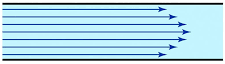
\includegraphics[scale=0.8]{Flujo_02_Laminar.png}
    \end{figure}
    \begin{tasks}(4)
        \task laminar
        \task turbulento
        \task seccionado
        \task estático
    \end{tasks}
    \question \textbf{(1 punto)} El número de Reynolds es una cantidad adimensional que nos indica cuándo un flujo \rule{2cm}{0.1mm} pasa a ser un flujo \rule{2cm}{0.1mm}.
    \begin{tasks}
        \task laminar - seccionado
        \task estático - turbulento
        \task laminar  - turbulento
        \task turbulento - laminar
    \end{tasks}
    
    \section{(9 puntos) Electricidad.}

    \question \textbf{(1 punto)} El flujo de las partículas cargadas en un conductor es lo que se conoce como \rule{2cm}{0.1mm}.
    \begin{tasks}(4)
        \task Resistencia.
        \task Voltaje.
        \task Potencia.
        \task Corriente.
    \end{tasks}
    \question \textbf{(1 punto)} Relaciona las unidades de las siguientes cantidades, una columna con la otra.
    \\
    \begin{minipage}[t]{0.4\linewidth}
        \begin{enumerate}[label=\arabic*)]
            \item Voltaje.
            \item Resistencia.
            \item Corriente.
        \end{enumerate}
    \end{minipage}
    \begin{minipage}[t]{0.4\linewidth}
        \begin{enumerate}[label=\alph*)]
            \item Ohm (\si{\ohm})
            \item Watt (\si{\watt})
            \item Ampere (\si{\ampere})
            \item Volt (\si{\volt})
        \end{enumerate}
    \end{minipage}
    \begin{tasks}(4)
        \task 1-d, 2-b, 3-a
        \task 1-a, 2-d, 3-c
        \task 1-d, 2-a, 3-c
        \task 1-a, 2-c, 3-b
    \end{tasks}
    \question \textbf{(1 punto)} \label{Problema_02} \textbf{Ejercicio de ejecución: } Determina la intensidad de la corriente eléctrica a través de una resistencia de \SI{150}{\kilo\ohm} al aplicarle una diferencia de potencial de \SI{220}{\volt}.
    \begin{tasks}(4)
        \task \SI{1.466}{\milli\ampere}
        \task \SI{1.966}{\ampere}
        \task \SI{2.066}{\milli\ampere}
        \task \SI{2.066}{\ampere}
    \end{tasks}
    \question \textbf{(1 punto)} En el siguiente circuito eléctrico se tienen $n$ resistencias del mismo valor conectadas en serie, ¿cuál es el valor de la resistencia total $(R_{T})$ del circuito entre los puntos $A^{\prime}$ y $B^{\prime}$?
    \begin{center}
    \begin{circuitikz}[american voltages]
        \draw 
            (0, 0) node [anchor=east] {$A^{\prime}$}
            to[short, o-] (1, 0)
            % (0, 0) to[V=10V] (0, 4)
            to [R, l=\mbox{$R$}] (3, 0)
            to [R, l=\mbox{$R$}] (5, 0)
            to [R, l=\mbox{$R$}] (7, 0)
            -- (8.5, 0) node[midway,fill=white,inner sep=5,scale=1.2] {$.\,.\,.$} (10.5, 0)
            ;
            \draw (8.5, 0) to [R, l=\mbox{$R$}] (10.5, 0)
                to[short, -o] (12, 0)
                node [anchor=west] {$B^{\prime}$};
    \end{circuitikz}  
    \end{center}
    \begin{tasks}(4)
        \task $R_{T} = n^{2} \, R$
        \task $R_{T} = n + R$
        \task $R_{T} = n \, R$
        \task $R_{T} = \dfrac{R}{n}$
    \end{tasks}
    \question \textbf{(1 punto)} En un circuito serie $RC$, se tiene que $R = \SI{5}{\kilo\ohm}$ y $C = \SI{3}{\micro\farad}$. ¿Cuál es la constante de tiempo del circuito?
    \begin{tasks}(4)
        \task \SI{15}{\second}
        \task \SI{1.5d-3}{\second}
        \task \SI{0.015}{\second}
        \task \SI{0.35}{\second}
    \end{tasks}
    \question \textbf{(1 punto)} En un circuito \rule{2cm}{0.1mm} la corriente se adelanta \ang{90} con respecto al voltaje:
    \begin{tasks}(4)
        \task $R \, C$
        \task $R \, L$
        \task $R \, L \, C$
        \task $R$
    \end{tasks}
    \question \textbf{(1 punto)} \label{Problema_03} \textbf{Ejercicio de ejecución: } Calcula la reactancia inductiva del siguiente inductor:
    \begin{center}
        \begin{circuitikz}[american voltages]
            \draw 
                (0, 0) to[short, o-] (1, 0)
                to [L, l=\mbox{$L=\SI{1.2}{\henry}$}] (3, 0)
                to[short, -o] (4, 0);
            \node at (2, -0.75) {$\omega = \SI{377}{\radian\per\second}$};
        \end{circuitikz}  
    \end{center}
    \begin{tasks}(4)
        \task \SI{500.9}{\ohm}
        \task \SI{452.4}{\ohm}
        \task \SI{370.7}{\ohm}
        \task \SI{246.1}{\ohm}
    \end{tasks}
    \question \textbf{(1 punto)} En un circuito en serie una resistencia $R = \SI{8}{\ohm}$ y un inductor $L = \SI{0.02}{\henry}$ están conectados a una fuente de voltaje $v = \num 283 \, \sin 300 \, t$ Volts. ¿Cuál es el valor de la impedancia compleja?
    \begin{tasks}(4)
        \task $Z {=} \SI{16}{\ohm} + j \, \SI{16}{\ohm}$
        \task $Z {=} \SI{16}{\ohm} - j \, \SI{16}{\ohm}$
        \task $Z {=} \SI{8}{\ohm} - j \, \SI{6}{\ohm}$
        \task $Z {=} \SI{8}{\ohm} + j \, \SI{6}{\ohm}$
    \end{tasks}
    \question \textbf{(1 punto)} Una resistencia $R = \SI{27.5}{\ohm}$ y un capacitor $C = \SI{66.7}{\micro\farad}$ se conectan en serie. La diferencia de potencial es $V = \num{50} \, \cos 1500 \, t$ \, Volts. ¿Cuál es la magnitud de la impedancia $Z$?
    \begin{tasks}(4)
        \task \SI{14.99}{\ohm}
        \task \SI{980.95}{\ohm}
        \task \SI{32.32}{\ohm}
        \task \SI{224.70}{\ohm}
    \end{tasks}

\end{questions}

\vspace*{1cm}
\textbf{\huge{Formulario.}}
\begin{table}[H]
    \centering
    \setlength{\tabcolsep}{40pt}
    \renewcommand{\arraystretch}{2.5}
    \begin{tabular}{c  c}
        \multicolumn{2}{c}{Hidrodinámica} \\
        $G = \dfrac{V}{t}$ & $G = A \, v$ \\
        $\text{Flujo} = \dfrac{m}{t}$ & $\text{Flujo} = \dfrac{\rho \, V}{t}$ \\
        $\text{Flujo} = G \, \rho$ & \\
        $v_{1} \, A_{1} = v_{2} \, A_{2}$ & $v = \sqrt{2 \, g \, h}$ \\
        \multicolumn{2}{c}{$P_{1} + \rho \, g \, h_{1} + \dfrac{1}{2} \rho \, v_{1}^{2} = P_{2} + \rho \, g \, h_{2} + \dfrac{1}{2} \rho \, v_{2}^{2}$} \\ \hline
        \multicolumn{2}{c}{Electricidad} \\
        $V = I \, R$ & $R_{T} = R_{1} + R_{2} + R_{3} + \ldots$ \\
        $\dfrac{1}{R_{T}} = \dfrac{1}{R_{1}} + \dfrac{1}{R_{2}} + \dfrac{1}{R_{3}} + \ldots$ & $\tau = R \, C$ \\
        $X_{C} = \dfrac{1}{\omega \, C}$ & $X_{L} = \omega\, L$ \\
        $Z = R + j \, X_{L}$ & $Z = R - j \, X_{C}$ \\
        $\abs{Z} = \sqrt{R^{2} + (X_{L})^{2}}$ & $\abs{Z} = \sqrt{R^{2} + (X_{C})^{2}}$ \\
\end{tabular}
\end{table}

\newpage

En este espacio deberás de incluir el desarrollo completo de los Problemas de Ejecución. El problema se califica de la siguiente manera: \textbf{a) Datos: 0.25 puntos}, \textbf{b) Expresión(es): 0.25 puntos}, \textbf{c) Sustitución: 0.25 puntos} y \textbf{d) Manejo de unidades: 0.25 puntos}.

\vspace*{0.5cm}
Solución al Problema de Ejecución \ref{Problema_01}:

\vspace*{4cm}
\rule{0.9\textwidth}{0.3mm}

Solución al Problema de Ejecución \ref{Problema_02}:

\vspace*{4.5cm}
\rule{0.9\textwidth}{0.3mm}

Solución al Problema de Ejecución \ref{Problema_03}:


\end{document}